\begin{figure}[ht]
  \caption{Cern data flow from collisions to analysis}
  \label{img:}
  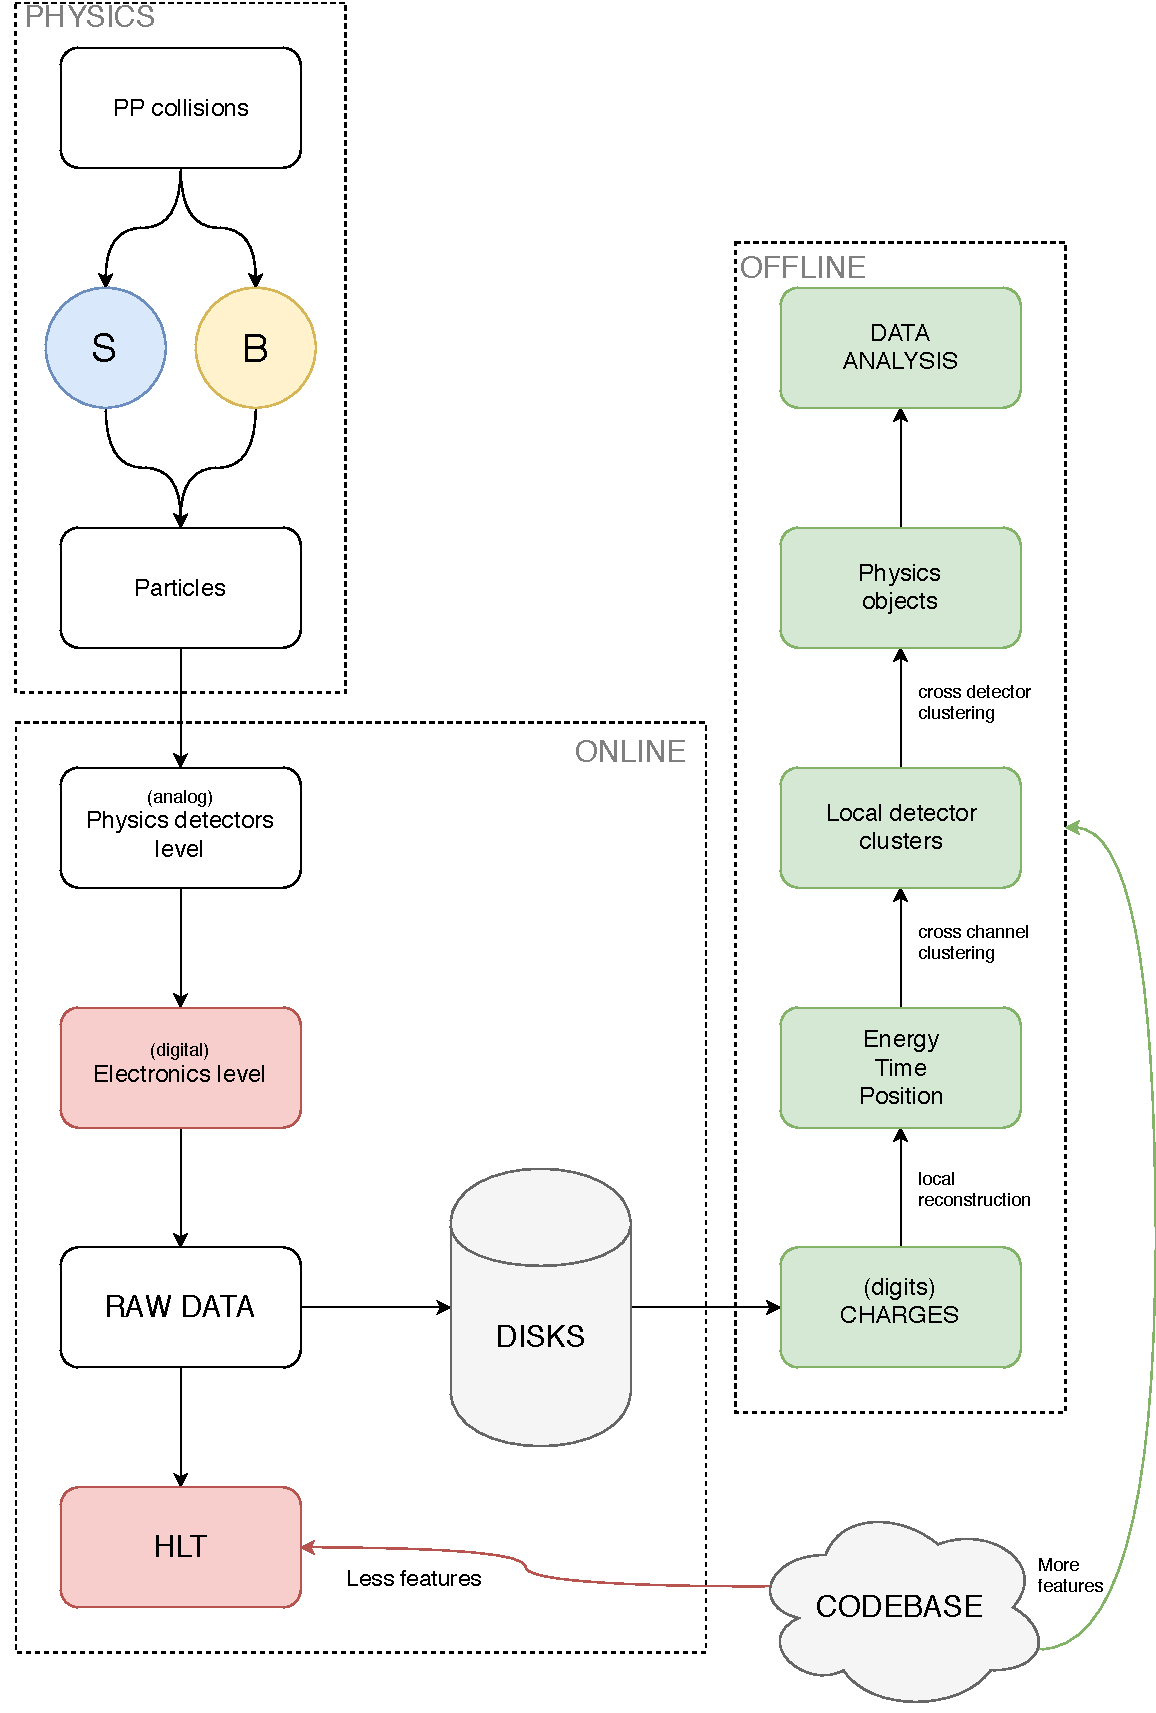
\includegraphics[height=\textheight]{img/dataflow}
\end{figure}
% This might be an introduction
Modern high energy physics (HEP) requires big data analysis. To make it possible several large scale objects are needed: from accelerators, detectors, data centers to the thousands of people involved to design and run the infrastructure. Here at CERN everything starts with physics by colliding particles and everything ends with the physics performed by analyzing the data acquired. But, to produce the necessary data, in the right amount, a long and complicated process is involved. It is worth to briefly describe it to understand the reason of our work and where is it place inside it. \\
\paragraph{Data generation}
